\section{Results}
\label{sec:results}
Figure \ref{fig:EMvsMCS} shows the expectation values for the energy and absolute magnetisation as a function of Monte Carlo sweeps with both an ordered and unordered initial configuration. Results for a low temperature 1.0 and a higher temperature 2.4, which is above the critical temperature, are shown. One can see that the expectation values stabilizes almost immediately when an ordered starting configuration is chosen for the lower temperature. But when an unordered configuration is chosen, the values does not stabilize until about $25000$ $mcs$. As for the higher temperature, both an ordered and unordered initial configuration gives a result that stabilizes quite fast, with some fluctuations, around a value. This happens after about 5000 $mcs$ for the energy, and after about 10000 $mcs$ for the magnetisation.   
\begin{figure}[htbp]
	\centering
	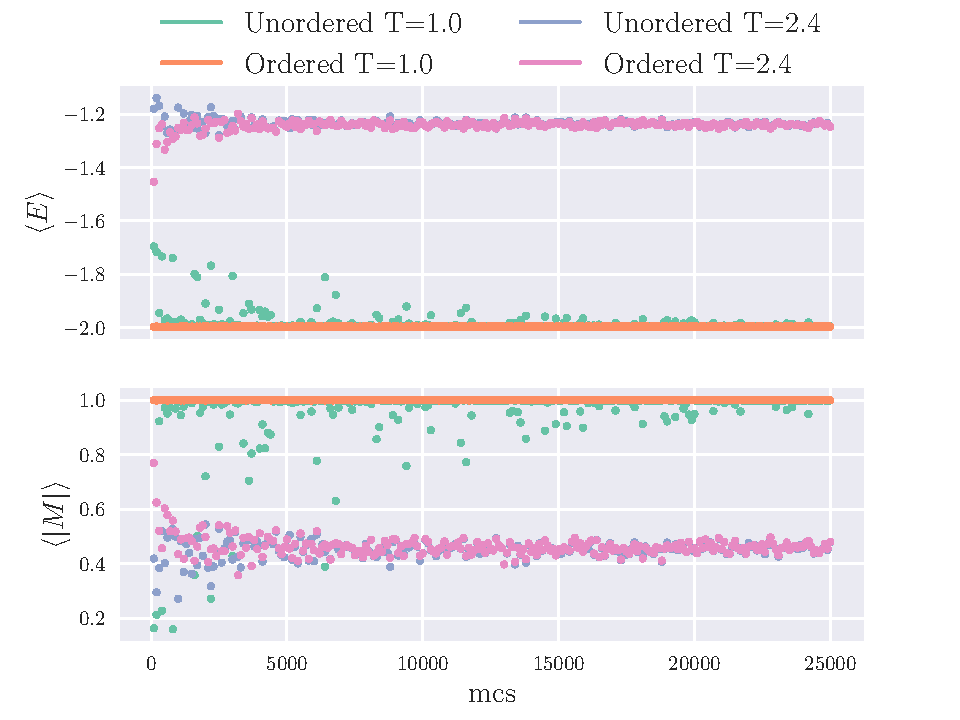
\includegraphics[width=0.5\textwidth]{EMvsMCS.pdf}
	\caption{Plot over expectation values for energy $E$ per spin and absolute magnetisation $|M|$ per spin as a functions of Monte Carlo sweeps $mcs$. The expectation values are plotted for $T=1.0$ and $T=2.4$ with both an ordered and unordered initial state.}
	\label{fig:EMvsMCS}
\end{figure}

\begin{figure}[htbp]
	\centering
	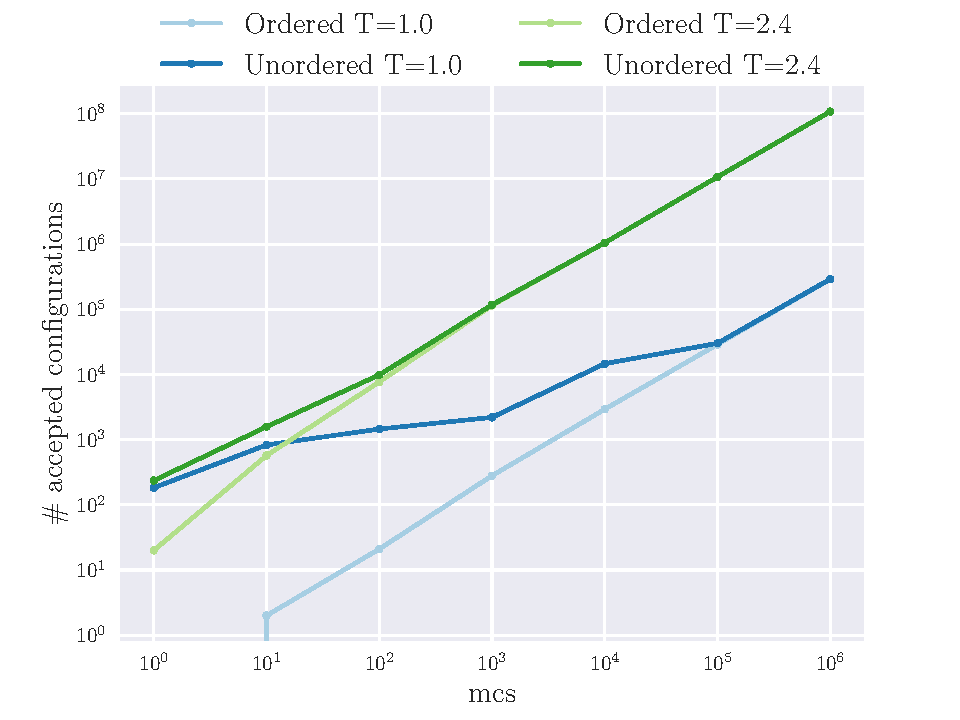
\includegraphics[width=0.5\textwidth]{nAccepted.pdf}
	\caption{Plot over the number of accepted configurations as a function of Monte Carlo sweeps $mcs$. The number of accepted configurations are plotted for $T=1.0$ and $T=2.4$ with both an ordered and unordered initial state. The scale is logarithmic.}
	\label{fig:nAccepted}
\end{figure}

\begin{figure}[htbp]
	\centering
	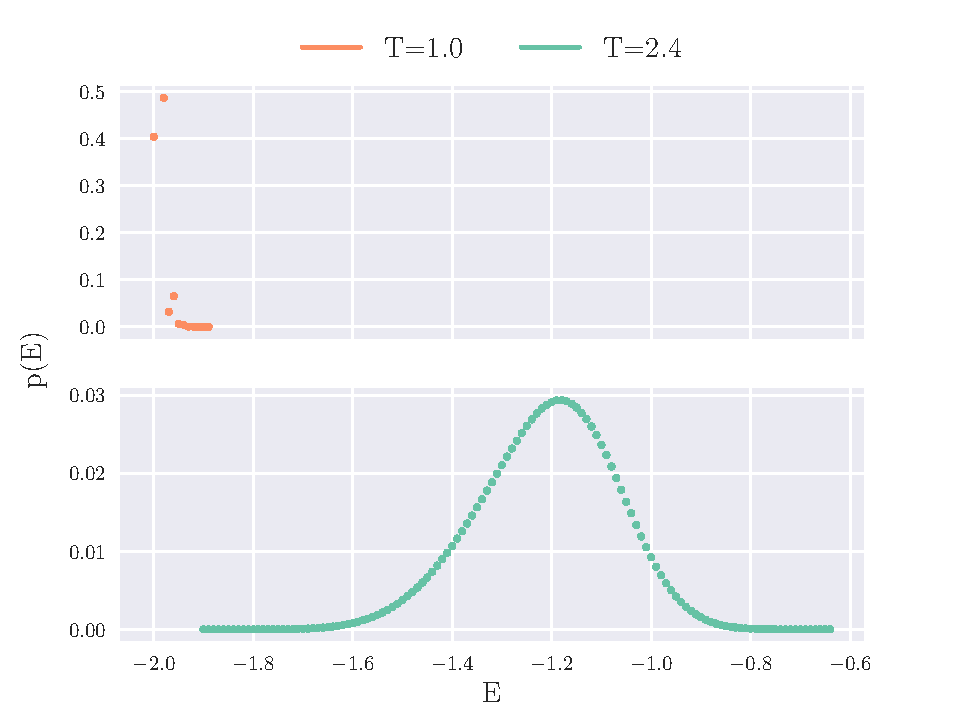
\includegraphics[width=0.5\textwidth]{probability.pdf}
	\caption{Plot over probabilities for a given energy $E$ per spin. The top plot is for temperature $T = 1.0$ while the bottom plot is for temperature $T=2.4$.}
	\label{fig:prob}
\end{figure}

\begin{table}[htbp]
	\centering
	\begin{tabular}{lll}
		T   & $\left\langle E\right\rangle$  & $\sigma^2$ \\
		\hline
		\addlinespace[0.1cm]
		1.0   & -1.997 & 0.025 \\
		2.4 & -1.237  & 8.116
	\end{tabular}
	\caption{Table over the expectation value  $\left\langle E\right\rangle$ and variation  $\sigma^2$ of the energy per spin after $10^6$ $mcs$ for temperatures $T=1.0$ and $T=2.4$.}
	\label{tab:prob}
\end{table}

\begin{figure}[htbp]
	\centering
	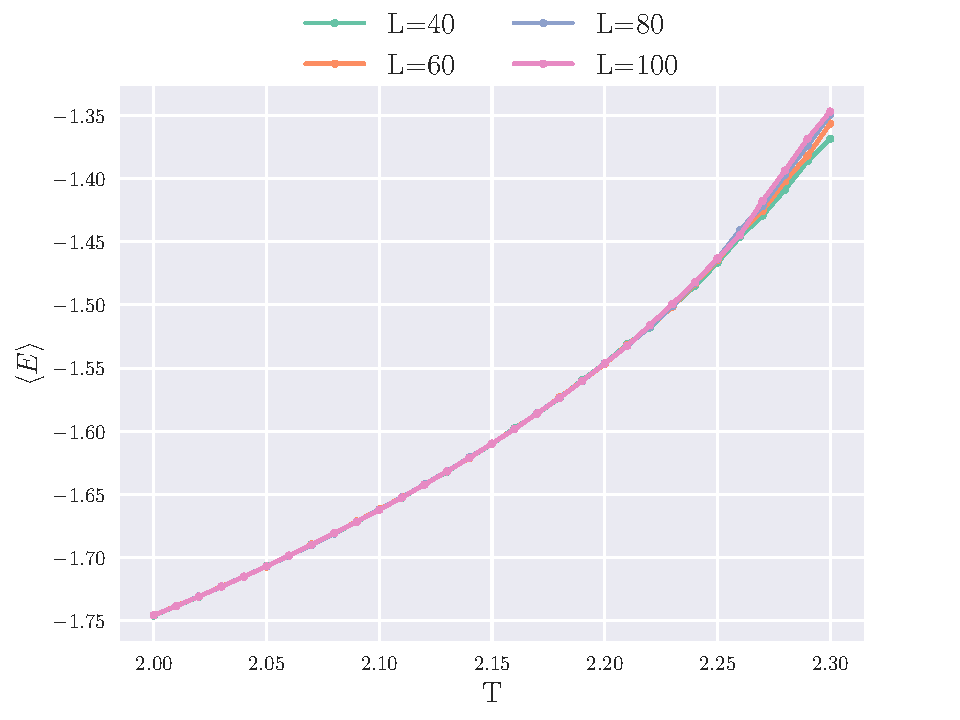
\includegraphics[width=0.5\textwidth]{energy.pdf}
	\caption{Plot over the expectation values for the energy per spin $\left\langle E\right\rangle$ as a function of temperature $T$ with step size $10^{-3}$. The results are from lattices with size $L=40,60,80$ and 100.  $10^6$ $mcs$ were used for each step.}
	\label{fig:E}
\end{figure}

\begin{figure}[htbp]
	\centering
	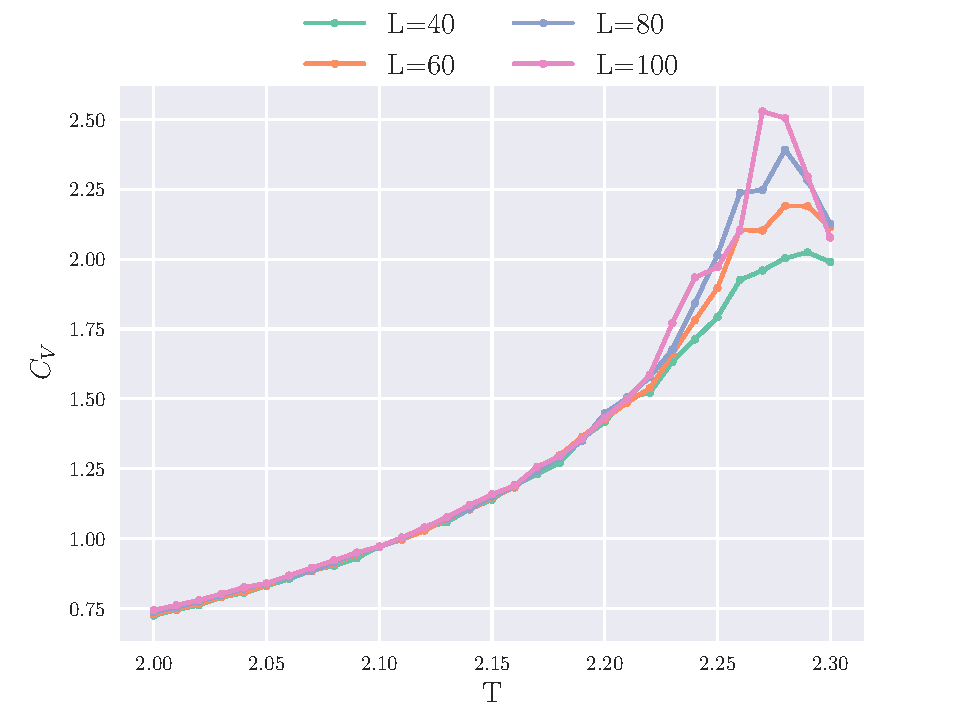
\includegraphics[width=0.5\textwidth]{heat_capacity.pdf}
	\caption{Plot over the expectation value for the absolute magnetisation per spin $\left\langle |M|\right\rangle$ as a function of temperature $T$ with step size $10^{-3}$. The results are from lattices with size $L=40,60,80$ and 100. $10^6$ $mcs$ were used for each step.}
	\label{fig:C}
\end{figure}

\begin{figure}[htbp]
	\centering
	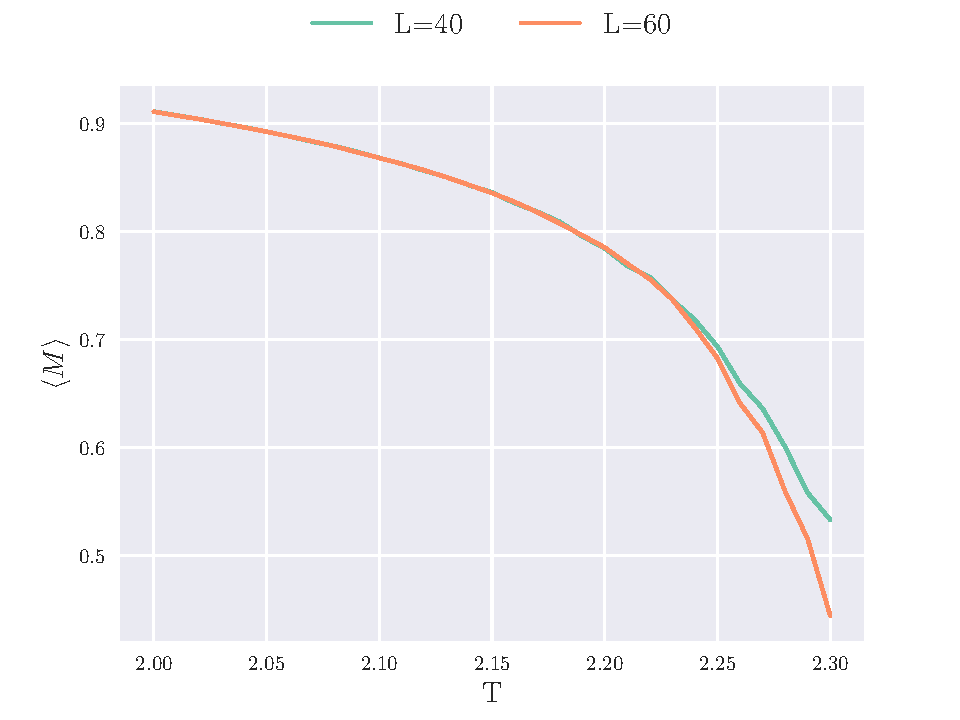
\includegraphics[width=0.5\textwidth]{magnetization.pdf}
	\caption{Plot over the expectation valuess for the specific heat per spin $C_V$ as a function of temperature $T$ with step size $10^{-3}$. The results are from lattices with size $L=40,60,80$ and 100. $10^6$ $mcs$ were used for each step.}
	\label{fig:M}
\end{figure}

\begin{figure}[htbp]
	\centering
	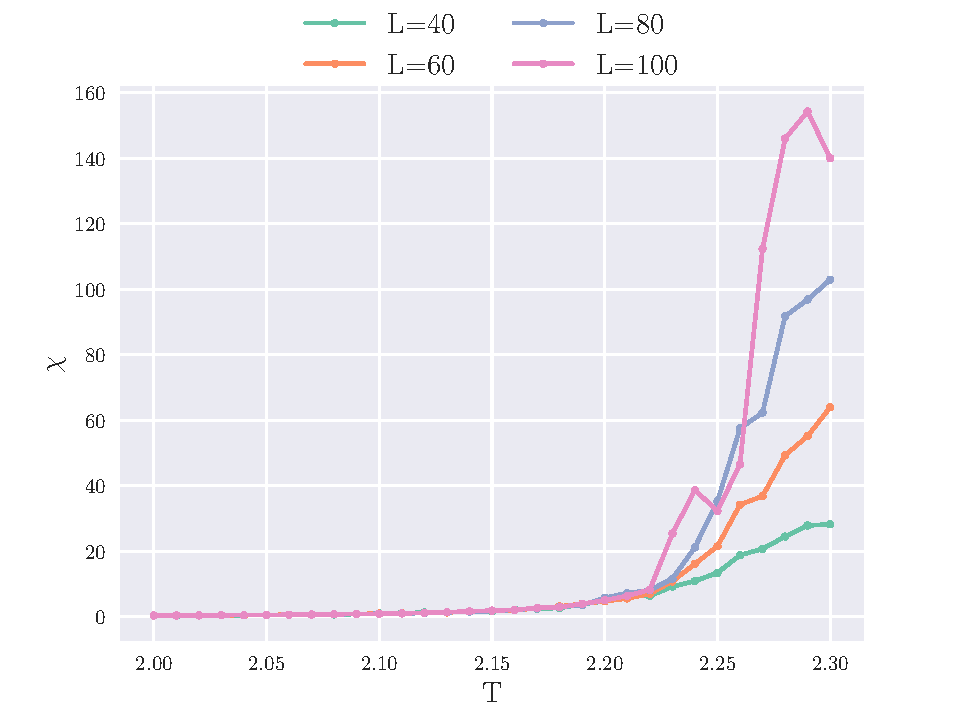
\includegraphics[width=0.5\textwidth]{susceptibility.pdf}
	\caption{Plot over the expectation values for the susceptibility per spin $\chi$ as a function of temperature $T$ with step size $10^{-3}$.The results are from lattices with size $L=40,60,80$ and 100. $10^6$ $mcs$ were used for each step.}
	\label{fig:Chi}
\end{figure}

\begin{figure}[htbp]
	\centering
	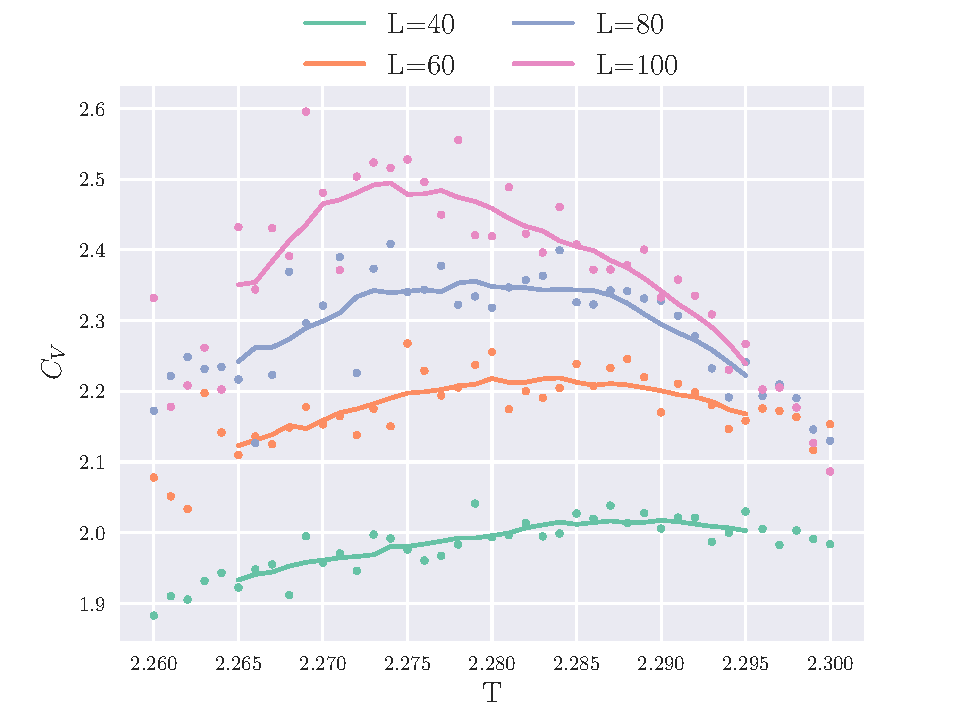
\includegraphics[width=0.5\textwidth]{zoom.pdf}
	\caption{Plot over the expectation values for the specific heat per spin $C_V$ as a function of temperature $T$ with step size $10^{-4}$.The results are from lattices with size $L=40,60,80$ and 100. $10^6$ $mcs$ were used for each step. The dots are the collected data, while the solid line is a running mean with a window size of 9.}
	\label{fig:zoom}
\end{figure}

